% !TEX program = XeLaTeX

\documentclass[12pt, letterpaper]{article}

\usepackage[l2tabu, orthodox]{nag}
\usepackage{tabu}
\usepackage[onehalfspacing]{setspace}
\usepackage{amsmath}
\usepackage{amsthm}
\usepackage{amsfonts}
\usepackage{float}
\usepackage{graphicx}
\usepackage{cmbright}
\usepackage{color}

%FONTS
\usepackage{fontspec}
\defaultfontfeatures{Mapping=tex-text}
\setmonofont{Fira Code}
\defaultfontfeatures{Extension = .otf}

\usepackage{listings}
\lstset{basicstyle=\footnotesize\ttfamily,breaklines=true}
% As a rule of thumb it should be loaded at the end of the preamble, after all
% the other packages. A few exceptions exist, such as the cleveref package that
% is also mentioned in this post. Hence, cleveref should be loaded after
% hyperref.
\usepackage{hyperref}
\definecolor{linkcolour}{rgb}{0.8,0.2,0.5}
\hypersetup{colorlinks,breaklinks,urlcolor=linkcolour, linkcolor=linkcolour}

% This package introduces the \cref command. When using this command to make
% cross-references, instead of \ref or \eqref, a word is placed in front of the
% reference according to the type of reference: fig. for figures, eq. for
% equations
\usepackage{cleveref}

\title{Report: Decision Tree}
\author{Hanlin He\footnote{hxh160630@utdallas.edu},
Tao Wang\footnote{txw162630@utdallas.edu}}

\begin{document}
\maketitle

% A brief report indicating any assumptions that you made, your best results, what you accomplished, and what you learned. The report should clearly indicate the names of the team members.
\section*{README}

The structure of the project please refer to the \texttt{README} file. An online `Github-style' rendering readme is \href{https://cs6375.github.io/DecisionTree/}{here}.

\section{Design}

There are mainly five class in the implementation.

\begin{itemize}
    \item \texttt{Instance}\\
    Represented a line of information in the data set file, including
    \begin{itemize}
        \item A list of boolean value, storing the values of each attribute in the instance. Currently only boolean type is supported.
        \item A boolean label, storing the label of the instance. Likely, only boolean type classification is supported currently.
    \end{itemize}

    \item \texttt{DataSet}\\
    Represented a dataset with only boolean attribute and boolean label, including
    \begin{itemize}
        \item A list of \texttt{Instance} instances.
        \item A list of \texttt{String} indicating the name of each attributes. Used ArrayList instead of array for the \texttt{indexOf} function. The variable is defined as \textbf{final} since the data set is fixed once read from file. No modification to current data set is allow. If a split operation is needed, allocate new data set to store new collection of instances.
        \item A list of boolean indicator to determine whether an attribute with certain index is excluded in computing.
        \item A int variable storing current \texttt{dimension} of the data set, i.e., the number of not-excluded attributes. Like the attribute above, intuitively, the \texttt{dimension} should be fixed once the data set was form.
    \end{itemize}

    \item \texttt{TrainingDataSet}\\
    Based on \texttt{DataSet} class, extended with entropy computation and split function. This class standalone because only the training data need compute entropy and split. Additionally, \texttt{TrainingDataSet} includes
    \begin{itemize}
        \item A double variable storing the entropy of current data set.
        \item A boolean label indicating the most common label at current level. This value is acquired alongside the entropy  calculation.
    \end{itemize}
    Note that, the \texttt{split()} operation do not modify current data set or any instances, it simply generate a new data set instance and assign the references of specific set of \texttt{Instance} instances to the new data set.

    \item \texttt{DecisionTreeNode}\\
    Represented a node in the decision tree, including
    \begin{itemize}
        \item A string label indicate the attribute used to split in this node.
        \item A boolean label indicate the most common class at current node. This value can be computed in building the tree. Although in internal node, the value is meaningless, it is very helpful in pruning, since no more computation is needed after pruning a subtree.
        \item A int value indicating the depth of current node.
        \item Left and Right reference of subtree.
        \item A boolean label indicating whether current node has been pruned. 
        \emph{Note that, in actual pruning, no reference pointing to the subtree is deleted. Only this boolean label is switched to \texttt{true}.} Since no actual modification is done to the tree, to recover the ``pruned'' subtree back, only operation needed is switch back this boolean label. It is relatively easy to calculate the accuracy of different ways of pruning.
    \end{itemize} 

    \item \texttt{DecisionTree}\\
    Represented a decision tree, including
    \begin{itemize}
        \item An \texttt{ArrayList} to store the whole tree in BFS order. Generated after the tree is constructed by the \texttt{DecisionTreeNode} of root. The first element is the root node.
        Note that, generally speaking, to store a tree, only the root of the tree is needed. This additional list does not modify the structure of the tree, yet it offers a much more convenient way to iterate thought the nodes in the tree. And more importantly, it gives indexes to the nodes, allowing random access, i.e., pruning the node randomly.
        \item An \texttt{ArrayList} to store all the leaf nodes according to BFS order. Generated alongside the \texttt{nodes}.
    \end{itemize}
\end{itemize}

\section{Pruning Method}

The pruning method was implemented based on \textbf{reduced-error pruning} on the text book, i.e., rather than randomly select and prune node, the program would 
\begin{enumerate}
    \item first iterate through all the node, 
    \item \emph{find the node whose removal most increases the decision tree accuracy over the validation set}, 
    \item removed it and continue with iteration until specified pruning factor is achieve or the tree has converged (no more node removal would increase the accuracy on the validation set).
\end{enumerate}

Based on this implementation, decision tree of \texttt{data sets 1} would eventually converge after 17 pruning and the accuracy increased from $74.3\%$ to $78.8\%$. Decision tree of \texttt{data sets 2} would eventually converge after 12 pruning and the accuracy increased from $76.7\%$ to $82.7\%$.

\section{Result}

The execution screen shot shown in \cref{s1} and \cref{s2}. The decision tree generated please refer to attached file \texttt{DecesionTree1.txt} and \texttt{DecesionTree2.txt}

\begin{figure}
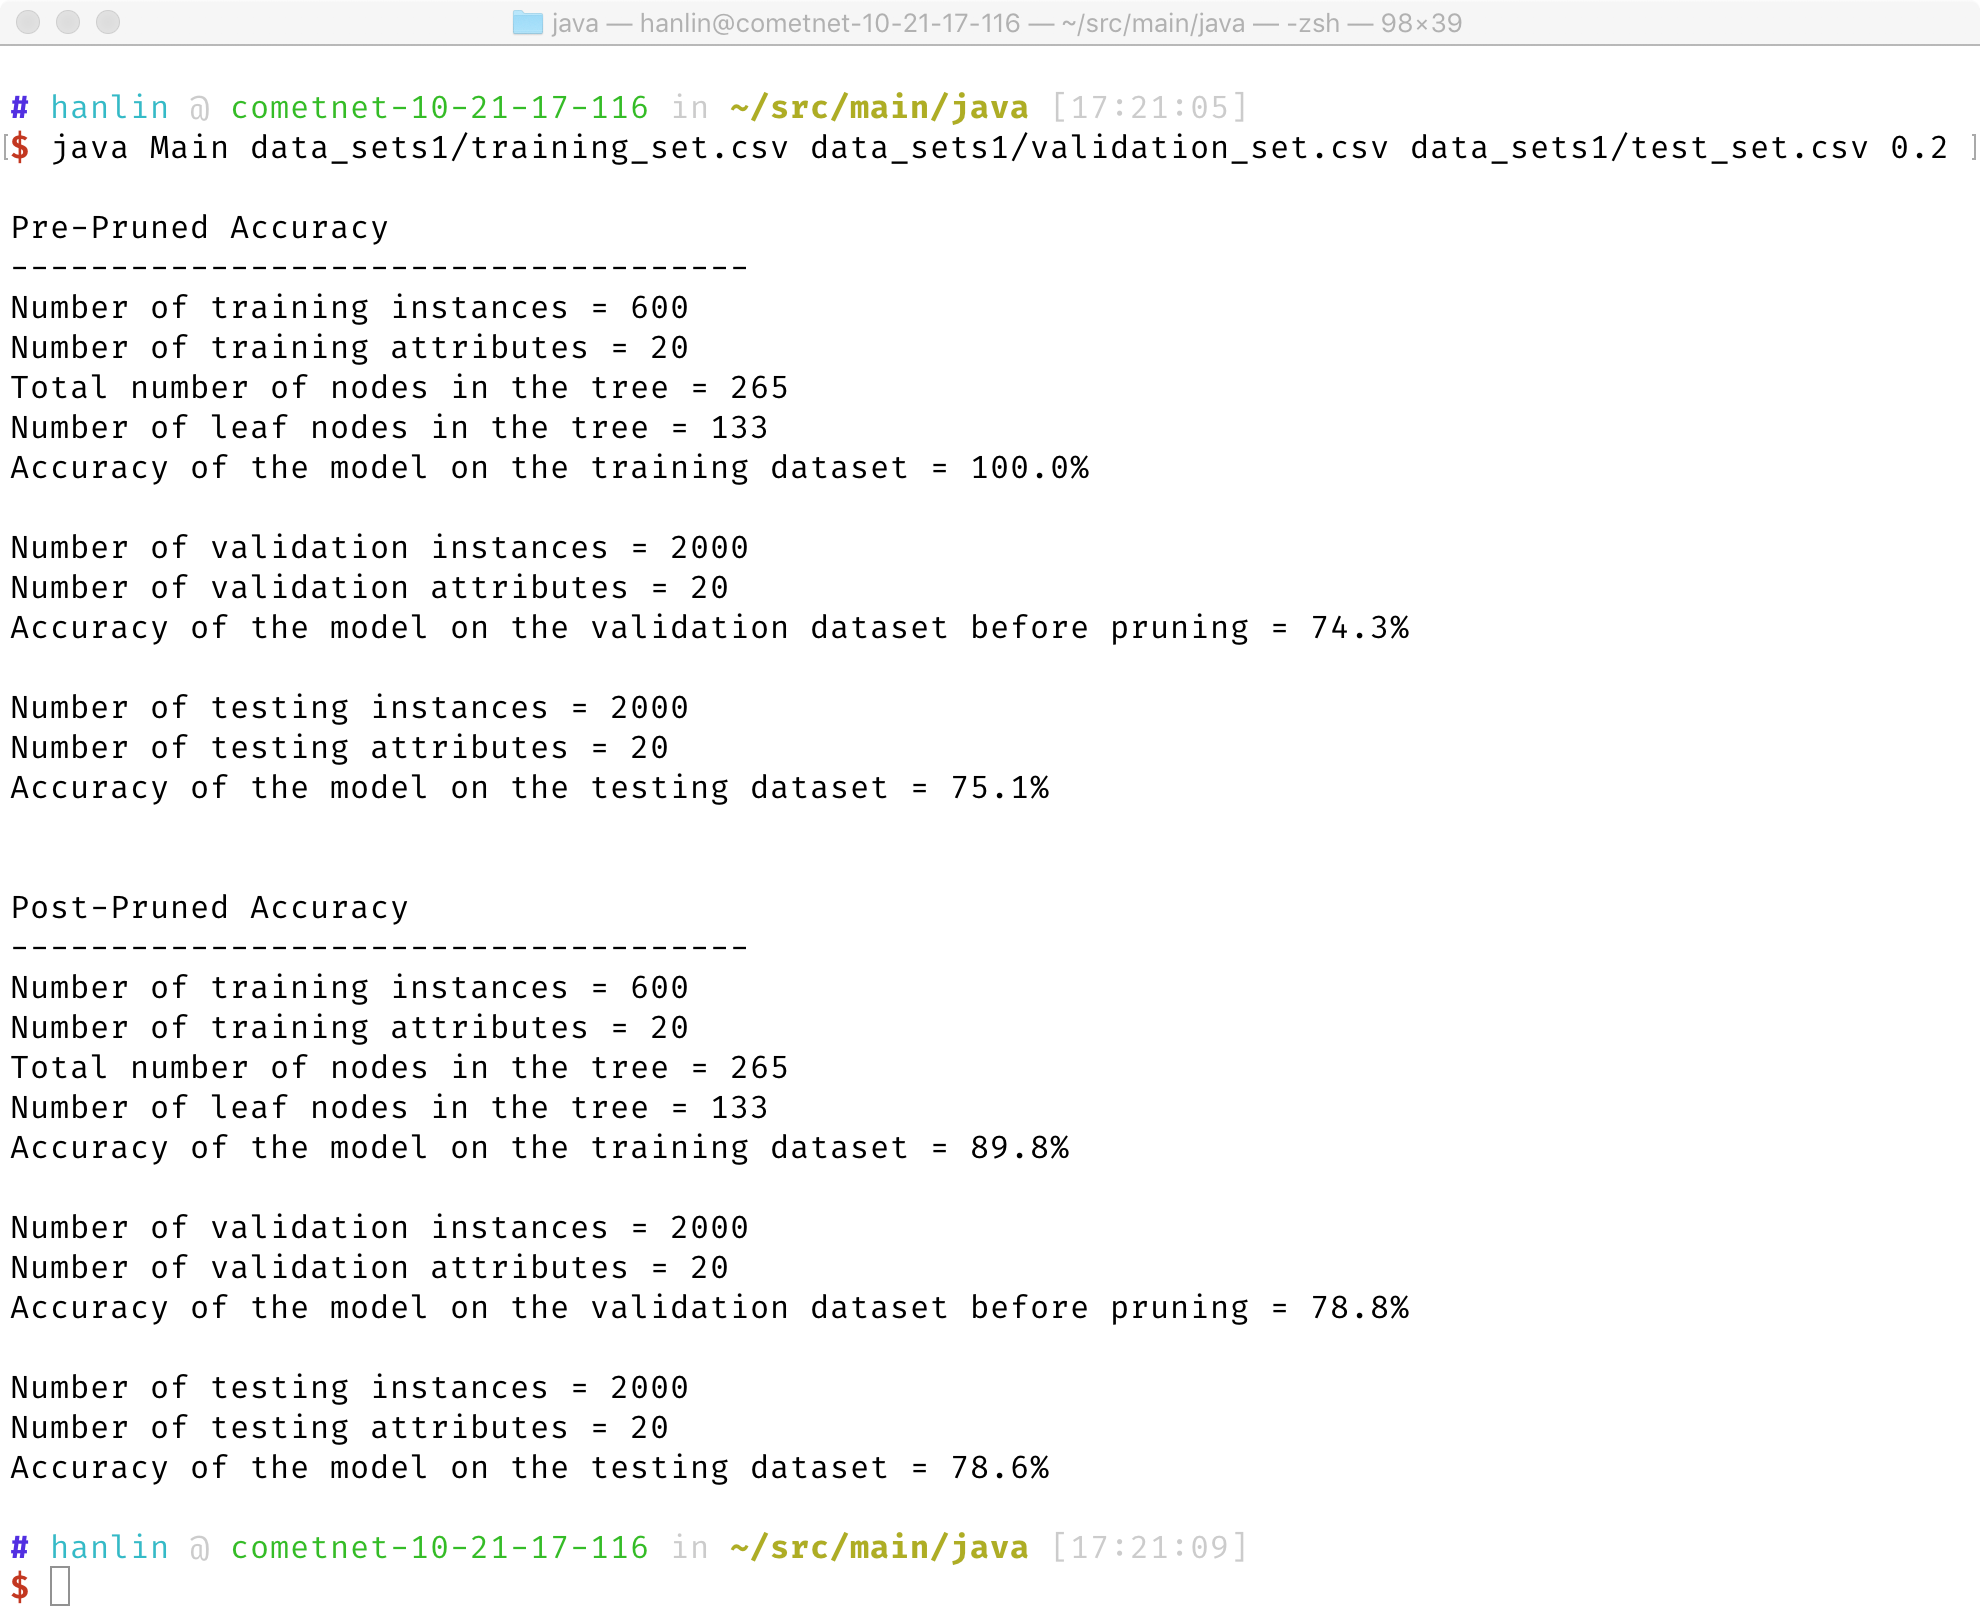
\includegraphics[width=\textwidth]{dataset1.png}
\caption{Execution for \texttt{Data Sets 1}}\label{s1}
\end{figure}

\begin{figure}
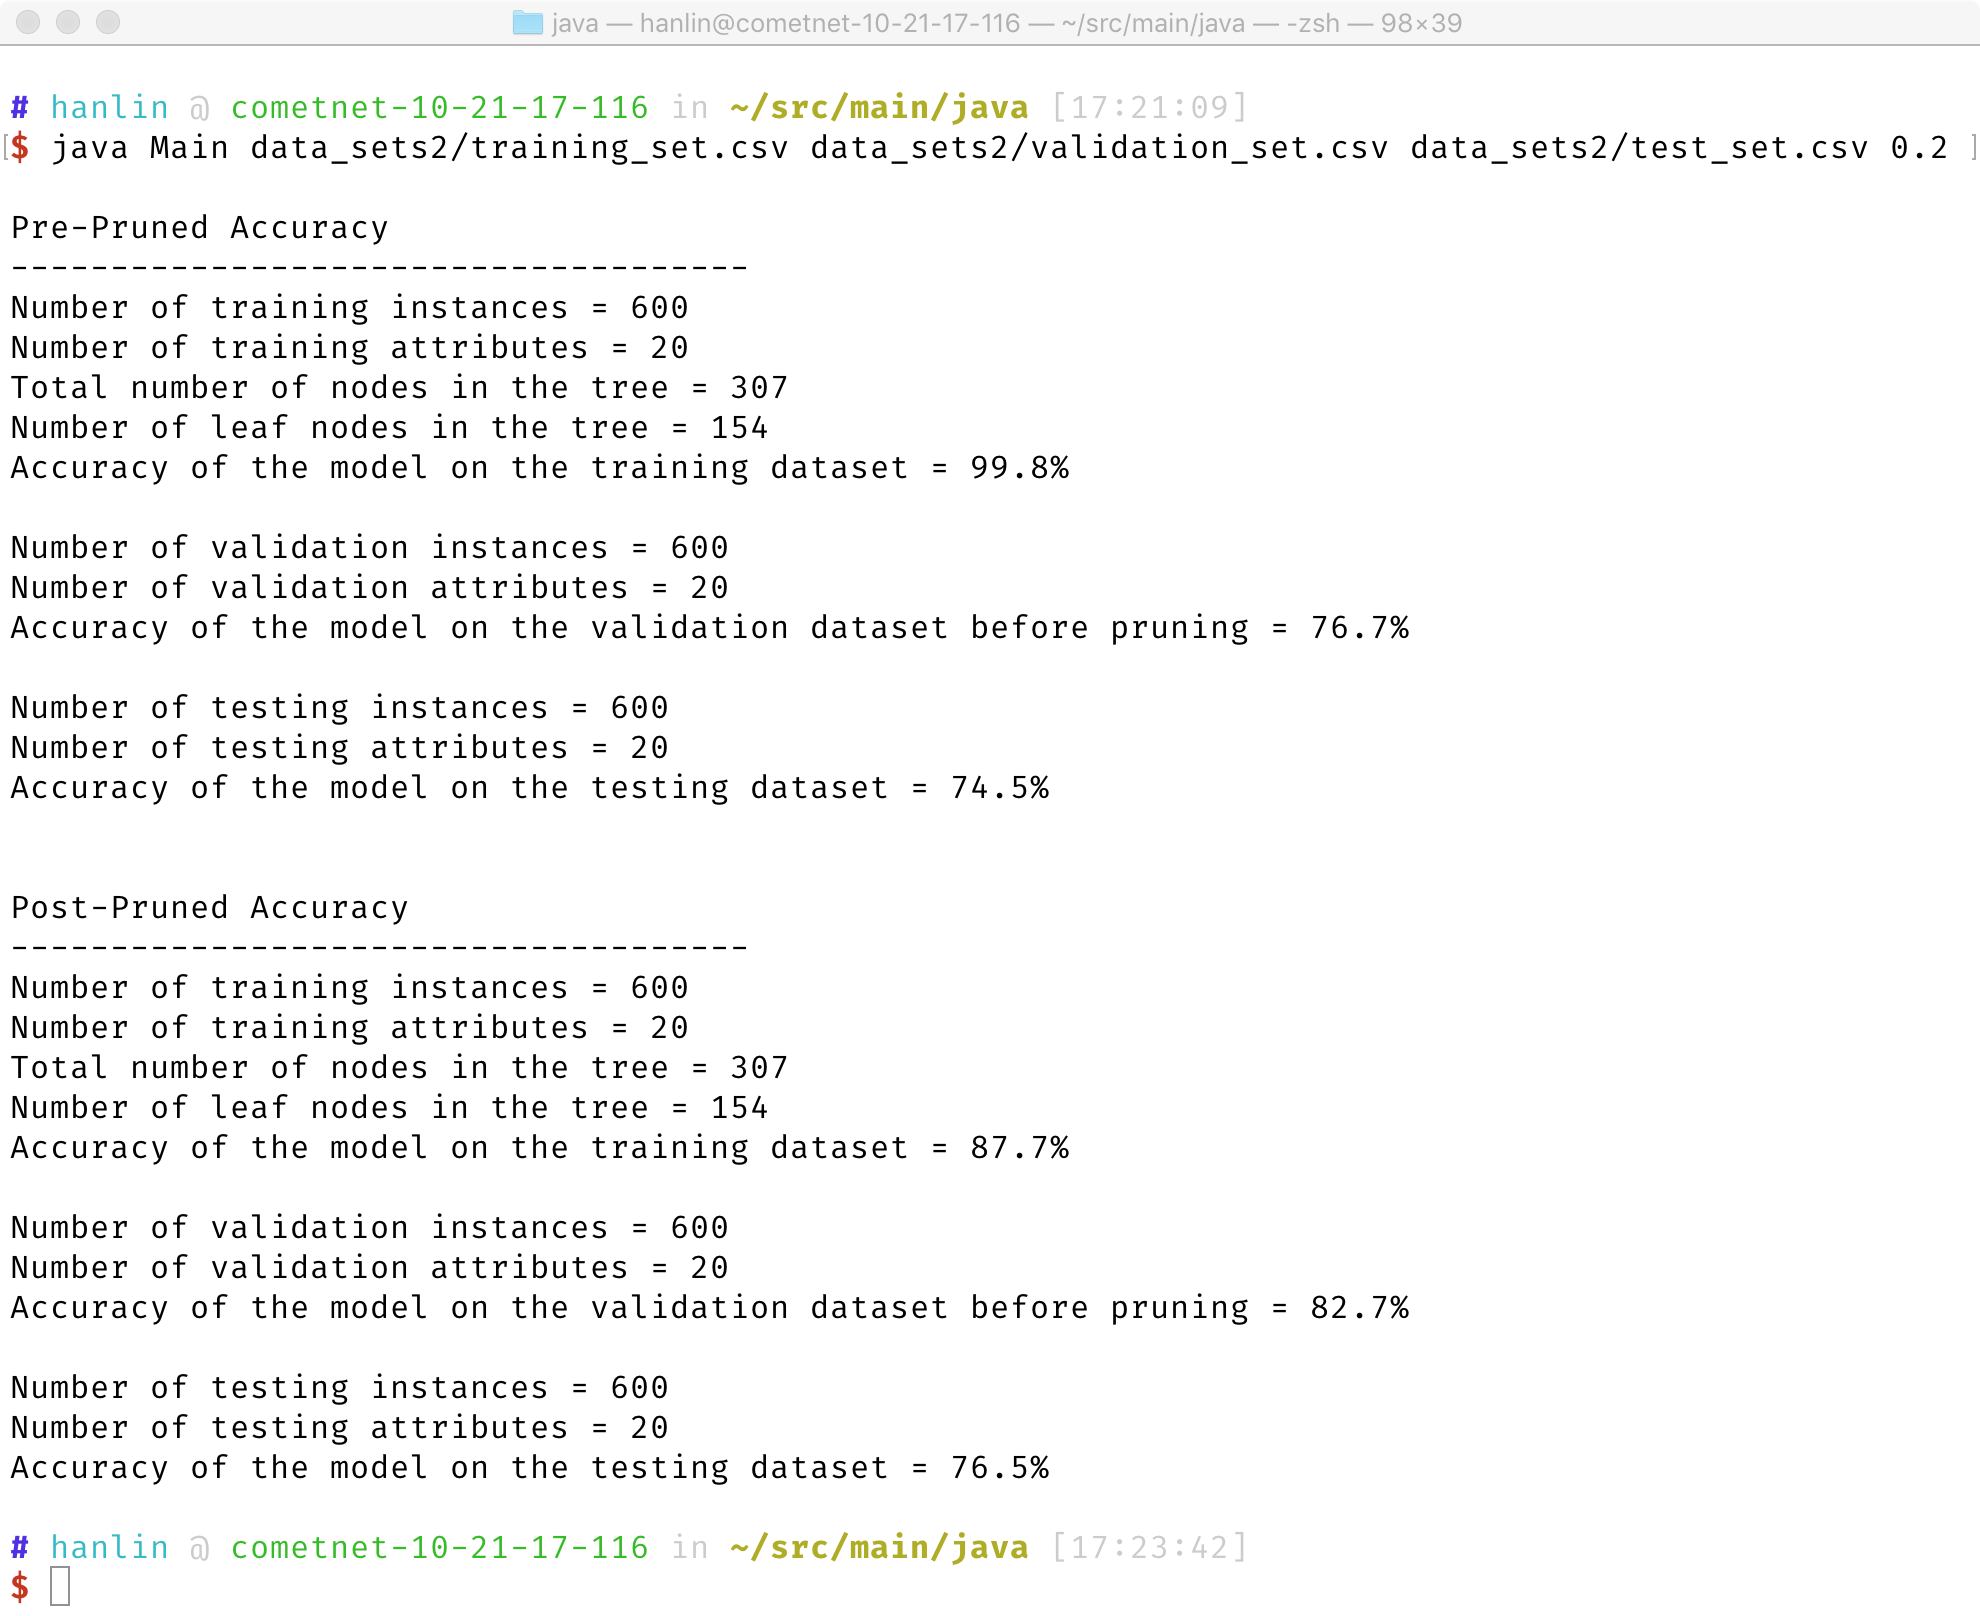
\includegraphics[width=\textwidth]{dataset2.png}
\caption{Execution for \texttt{Data Sets 2}}\label{s2}
\end{figure}



\end{document}
